\section{Theoretische Grundlagen} \label{sec:TheoretischeGrundlagen}

\subsection{EMI-Filter} \label{subsec:emifilter}
Das vorgegebene EMI-Filter muss bezüglich der Einfügungsverluste (insertion loss) untersucht werden. Die Einfügunsverluste hängen vom Gesamtrauschen der Schaltung ab. Es wird ein Ansatz verwendet, der in der Praxis weit verbreitet ist, bei welchem das Gesamtrauschen in zwei Komponenten unterteilt wird. Man spricht vom Gegen-(=Differential Mode=DM) und Gleichtaktrauschen (=Common Mode=CM). Anhand der vorgegebenen CM- und DM-Äquivalenten Schaltungen (Abbildungen \ref{fig:CM-Schaltungäquivalent}, \ref{fig:DM-Schaltungsäquivalent})werden die Einfügungsverluste in Funktion der Frequenz berechnet. Die Berechnungen decken einen Bereich von 0 bis 30MHz ab.

Die Einfügungsverluste sind wie folgt definiert: 

\begin{equation}\label{equ:Freqgang}
	IL = \left\lvert H(j\omega) \right\rvert = 20*log(\frac{ \left\lvert U_{20} \right\rvert }{ \left\lvert U_2 \right\rvert })
\end{equation}
In der Definition kann das Spannungsverhältnis durch den Streuparameter \ref{subsec:Streuparameter} (S-Parameter) S\textsubscript{21} ersetzt werden \ref{equ:Einfügungsverluste}.
\begin{equation}\label{equ:Einfügungsverluste}
	IL = -20*log (\left\lvert S_{21} \right\rvert)
\end{equation}
 Dieser Parameter \ref{equ:def_s21} beschreibt den Transmissionsgrad des Filters. Die Einfügungsverluste wären auch mit dem Verhältnis von eingehende zu abegegebene Leistung zu berechnen, jedoch eignet sich diese Methode mehr beim messtechnischen bestimmen der Einfügungsverluste. 
\newpage
\subsection{Schaltungen} \label{subsec:schaltungen}
Folgende Schaltungen stellen die CM- und DM-Äquivalenten Schaltungen. Da die Berechnungen in einem Bereich von bis zu 30 MHz gemacht werden, ist es notwendig die parasitären Parameter von Spule und Kondensator miteinzubeziehen.

\begin{figure}[H]
	\centering
	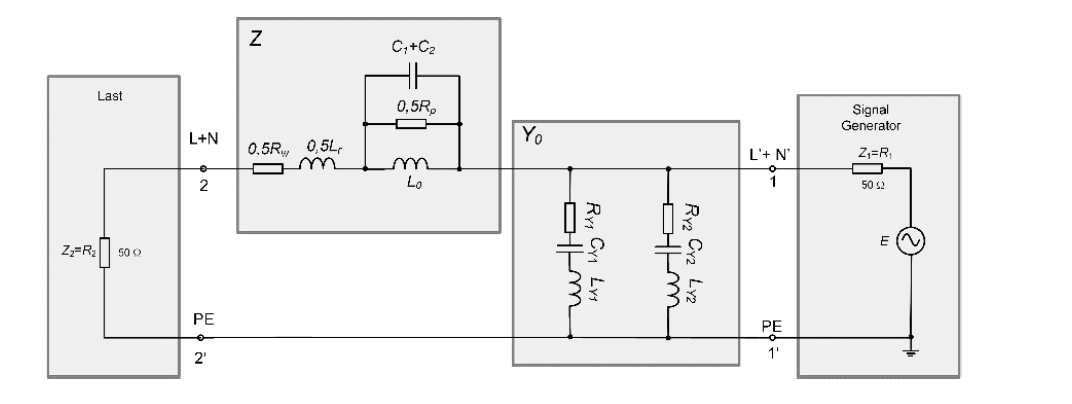
\includegraphics[width=15cm]{CM_ElectricalCircuit.png}
	\caption{CM-Schaltungäquvalent}
	\label{fig:CM-Schaltungäquivalent}
\end{figure}

\begin{figure}[H]
	\centering
	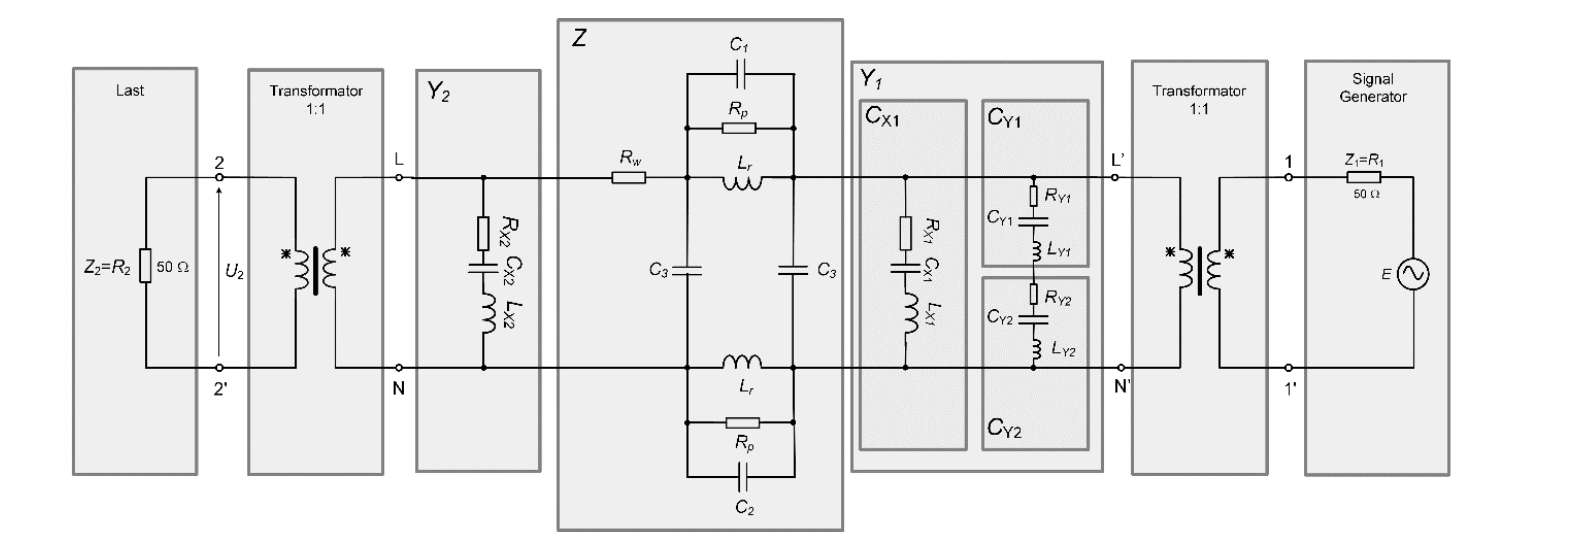
\includegraphics[width=15cm]{DM_ElectricalCircuit.png}
	\caption{DM-Schaltungsäquvalent}
	\label{fig:DM-Schaltungsäquivalent}
\end{figure}
\newpage
\subsection{Einfügungsverluste ermitteln} \label{subsec:vorgehen}
Die Einfügungsverluste werden analytisch ermittelt. Im ersten Schritt werden die Berechnungen in MATLAB gemacht. Somit können die Funktionen  geplottet werden. Diese Plots werden dann mit Simulationen in MPLAB Mindi verglichen um festzustellen ob diese korrekt sind. Die vollständigen und korrekten Berechnungen können somit in Java implementiert werden. Um die Einfügungsverluste bestimmen zu können, wird das Model der 2-Tore verwendet. Einzelne Schaltungsteile werden in ABCD-Matrixen\ref{ABCD-Matrix} abgebildet, welche dann durch Kaskadierung der einzelnen ABCD-Matrixen zusammengeführt werden. Die Einfügungsverluste werden aus den Streuparameter\ref{subsec:Streuparameter} abgeleitet, welche direkt aus der ABCD-Matrix berechnet werden.
Der S-Parameter S\textsubscript{21} gibt den Transmissionsgrad der Wellen an, die vom Tor 1 zum Tor2 übertragen wird. Die S-Parameter sind abhängig von den Bezugswiderständen (Innenwiderstand der Quelle sowie Lastwiderstand). In unserem Fall sind die Bezugswiderstände mit 50Ohm gegeben.

\newpage
\subsection{Streuparameter}\label{subsec:Streuparameter}
Die Streuparameter (S-Parameter) werden in der Hochfreqeunztechnik verwendet, um das Verhalten von n-Toren zu beschreiben. Bei einem 2-Tor sind vier Streuparameter von nöten um das Verhalten zu beschreiben. Sie beschreiben die Transmission von Tor 1 zu Tor 2, sowie von Tor 2 zu Tor 1. Des weiteren zeigen sie die Reflexion an den Toren auf. Abbildung \ref{fig:2-Tor} \nameref{fig:2-Tor} zeigt die Streuparameter an einem 2-Tor. 
\begin{figure}[H]
	\centering
	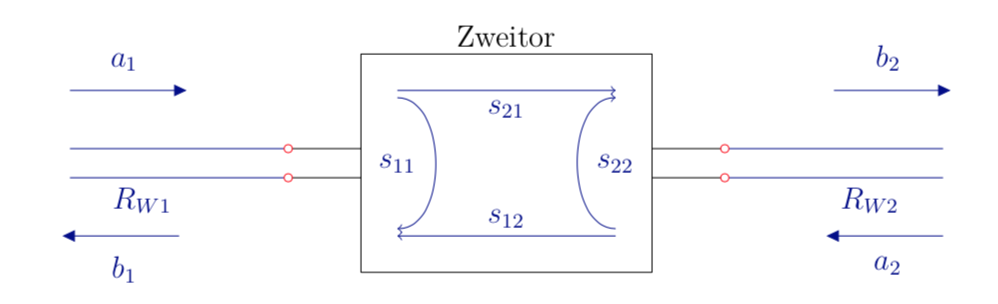
\includegraphics[width=15cm]{s_params_def.png}
	\caption{2-Tor Wellengrössen und Anschlussleitungen}
	\label{fig:2-Tor}
\end{figure}
Bei den S-Parameter werden die Eingangs- und Ausgangsgrössen nicht direkt anhand elektrischer Ströme und Spannungen beschrieben. Sie werden mithilfe von Wellengrössen beschrieben, wobei a\textsubscript{i} die einlaufenden Wellen sind und b\textsubscript{i} die Reflektierenden Wellen. Der Index i stellt den Torindex dar. Formel \ref{equ:def_a} und \ref{equ:def_b} zeigen wie die Wellengrössen a\textsubscript{i} sowie b\textsubscript{i} definiert sind.
\begin{equation}\label{equ:def_a}
	a_{ i } = \frac{ U_{ i}+R_{ Wi }I_{ i }}{2*\sqrt{ R_{ Wi } }}
\end{equation}
\begin{equation}\label{equ:def_b}
	b_{ i } = \frac{ U_{ i}-R_{ Wi }I_{ i }}{2*\sqrt{ R_{ Wi } }}
\end{equation}
Die Wellengrössen gelten nur für den gegebenen Bezugswiderstand R\textsubscript{Wi}. Der Bezugswiderstand kann einerseits der Innenwiderstand der angeschlossenen Quelle sein oder der Lastwiderstand der angeschlossenen Last.

Aus der Abbildung 2.3 lässt sich folgende Streumatrix darstellen:
\begin{equation}
	\left[
		\begin{matrix}b_1 \\ b_2 \end{matrix}
	\right]
 	=
 	\left[
 		\begin{matrix}
			s_{11}&s_{12} \\s_{21}&s_{22}
		\end{matrix}
	\right]
	* 
	\left[
		\begin{matrix}
			a_1\\b_2
		\end{matrix}
	\right]
\end{equation}
Die Elemente der S-Matrix sind:

\begin{equation}\label{equ:def_s11}
	s_{11} = b_1/a_1\textsf{ Eingangsreflexionsfaktor bei angepasstem Ausgang (a\textsubscript{2}=0)}
\end{equation}
\begin{equation}\label{equ:def_s12}
	s_{12} = b_1/a_2\textsf{ Rückwärtstransmissionsfaktor bei angepasstem Eingang (a\textsubscript{1}=0)}
\end{equation}
\begin{equation}\label{equ:def_s21}
	s_{21} = b_2/a_1\textsf{ Vorwärtstransmissionsfaktor bei angepasstem Ausgang (a\textsubscript{2}=0)}
\end{equation}
\begin{equation}\label{equ:def_s22}
	s_{22} = b_2/a_2\textsf{ Ausgangsreflexionsfaktor bei angepasstem Eingang (a\textsubscript{1}=0)}
\end{equation}
\newpage

\subsection{ABCD-Matrix}\label{ABCD-Matrix}
Die ABCD-Matrix ist eine weitere gängige Variante, um das Verhalten von 2-Toren zu beschreiben. Diese Variante hat den Vorteil, dass man in Serie 
geschaltene 2-Tore ohne grossen Aufwand zusammen rechnen kann. Sobald man die einzelnen ABCD-Matrixen gebildet hat und die Schaltung soweit vereinfacht ist, dass nur noch in Serie geschaltene ABDC-Matrixen vorzufinden sind, können diese miteinander multipliziert werden. Das Matrix-Produkt stellt dann die ABCD-Matrix der Gesamtschaltung dar. Folgende gängigen Schaltungen helfen die ABCD-Matrixen der einzelnen Schaltungsteilen zu bilden.

Die Längsimpedanz lässt sich anhand der ABCD-Matrix A\textsubscript{L} \ref{equ:horizImpedance} darstellen
\begin{figure}[H]
	\begin{minipage}[h]{0.45\linewidth}
		\centering
		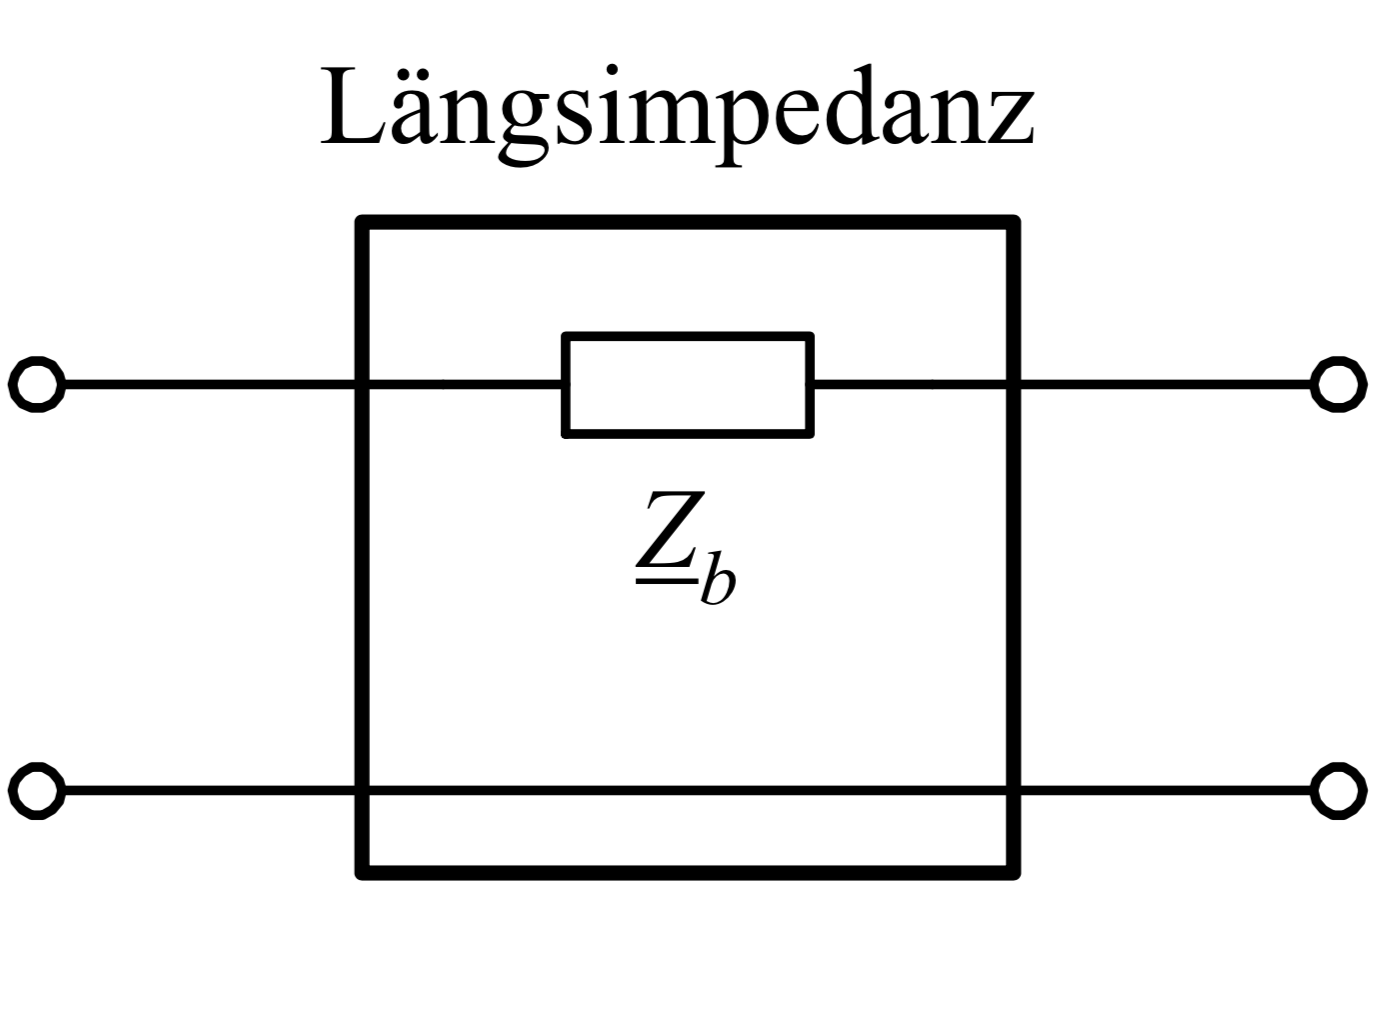
\includegraphics[width = 3cm]{h_impedance.png}
		\caption{Längsimpedanz}
	\end{minipage}
	\begin{minipage}[h]{0.45\linewidth}
		\centering
		\begin{equation}\label{equ:horizImpedance}
			A_L = \left[\begin{matrix}
			1&\underline{Z}_b\\0&1
			\end{matrix}\right]
		\end{equation}
	\end{minipage}
\end{figure}
Die Querimpedanz lässt sich anhand der ABCD-Matrix A\textsubscript{Q} \ref{equ:verticImpedance} darstellen
\begin{figure}[H]
	\begin{minipage}[h]{0.45\linewidth}
		\centering
		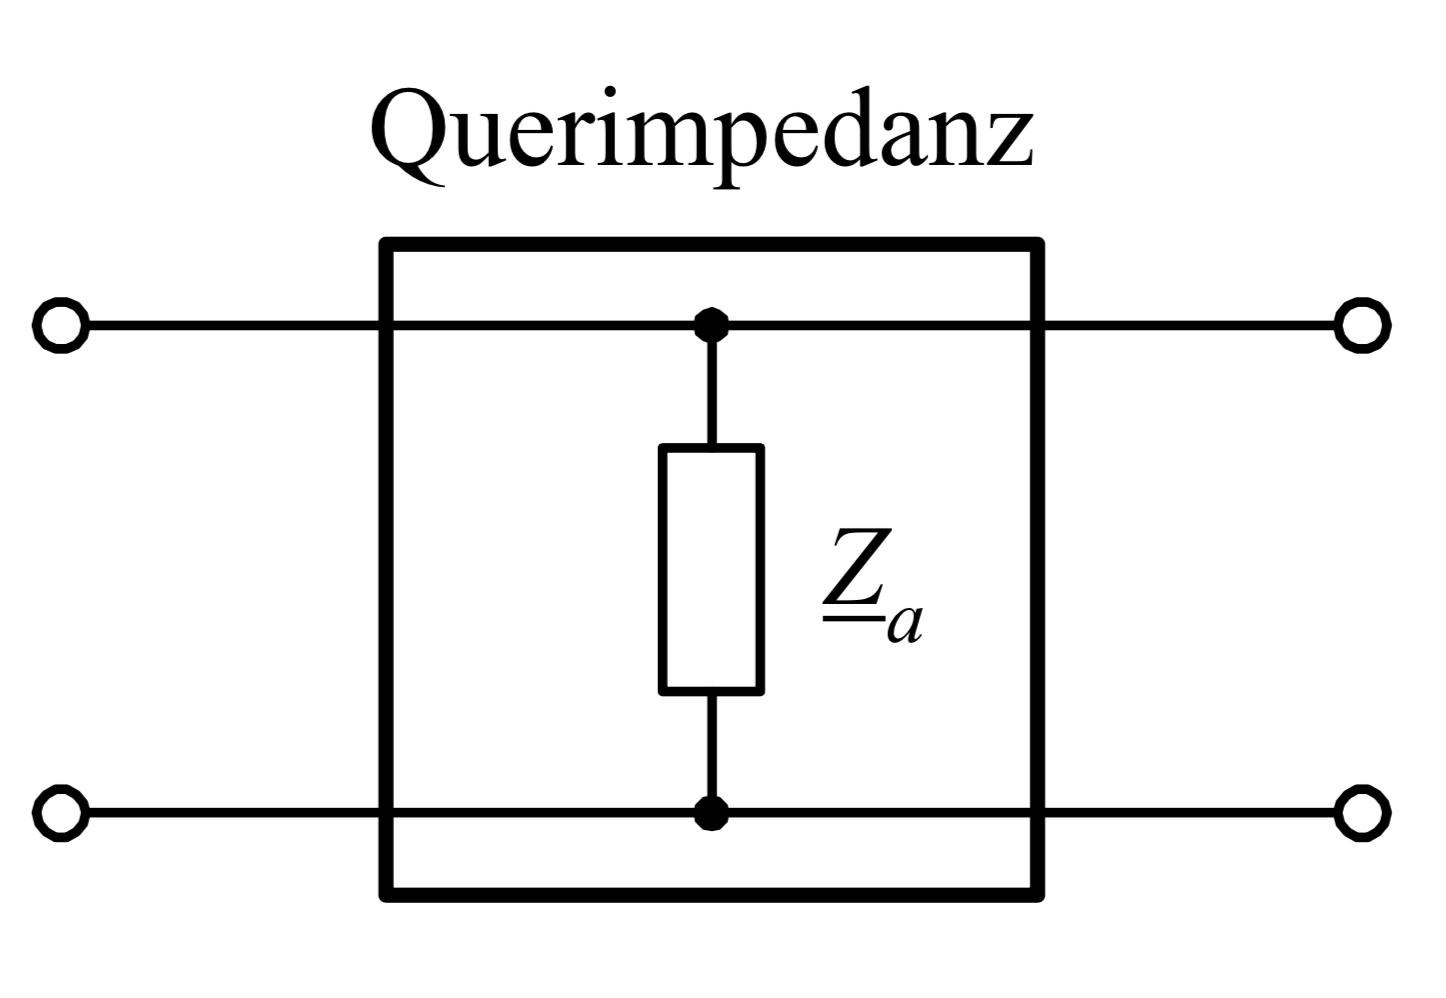
\includegraphics[width = 3cm]{v_impedance.png}
		\caption{Querimpedanz}
	\end{minipage}
	\begin{minipage}[h]{0.45\linewidth}
		\centering
		\begin{equation}\label{equ:verticImpedance}
			A_Q = \left[\begin{matrix}
			1&0\\\frac{1}{\underline{Z}_a}&1
			\end{matrix}\right]
		\end{equation}
	\end{minipage}
\end{figure}
Die Impedanz eines T-Glieds lässt sich anhand der ABCD-Matrix $A_T$ \ref{equ:tImpedance} darstellen
\begin{figure}[H]
	\begin{minipage}[h]{0.45\linewidth}
		\centering
		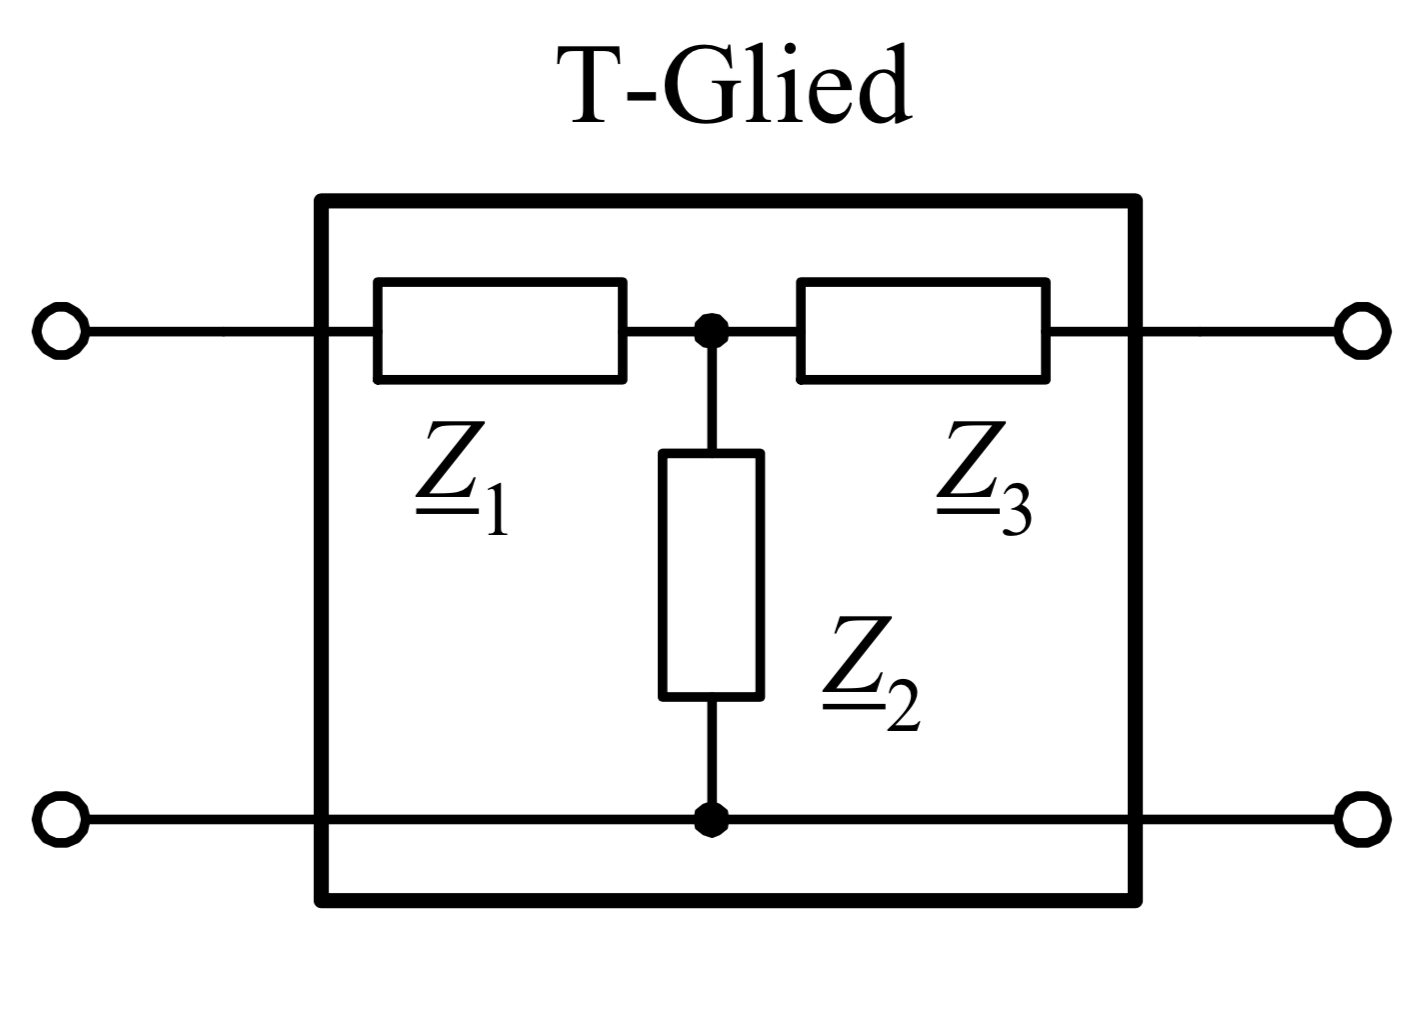
\includegraphics[width = 3cm]{t_impedance.png}\label{fig:tImpedance}
		\caption{T-Glied}
	\end{minipage}
	\begin{minipage}[h]{0.45\linewidth}
		\centering
		\begin{equation}\label{equ:tImpedance}
			A_T = \left[\begin{matrix}
			1+\frac{\underline{Z}_2}{\underline{Z}_3}&\underline{Z}_1+\underline{Z}_3+\frac{\underline{Z}_1\underline{Z}_3}{\underline{Z}_2}\\
			\frac{1}{\underline{Z}_2}&1+\frac{\underline{Z}_3}{\underline{Z}_2}
			\end{matrix}\right]
		\end{equation}
	\end{minipage}
\end{figure}
Die Impedanz eines  $\pi$-Glieds lässt sich anhand der ABCD-Matrix $A_\pi$   \ref{equ:piImpedance} darstellen
\begin{figure}[H]
	\begin{minipage}[h]{0.45\linewidth}
		\centering
		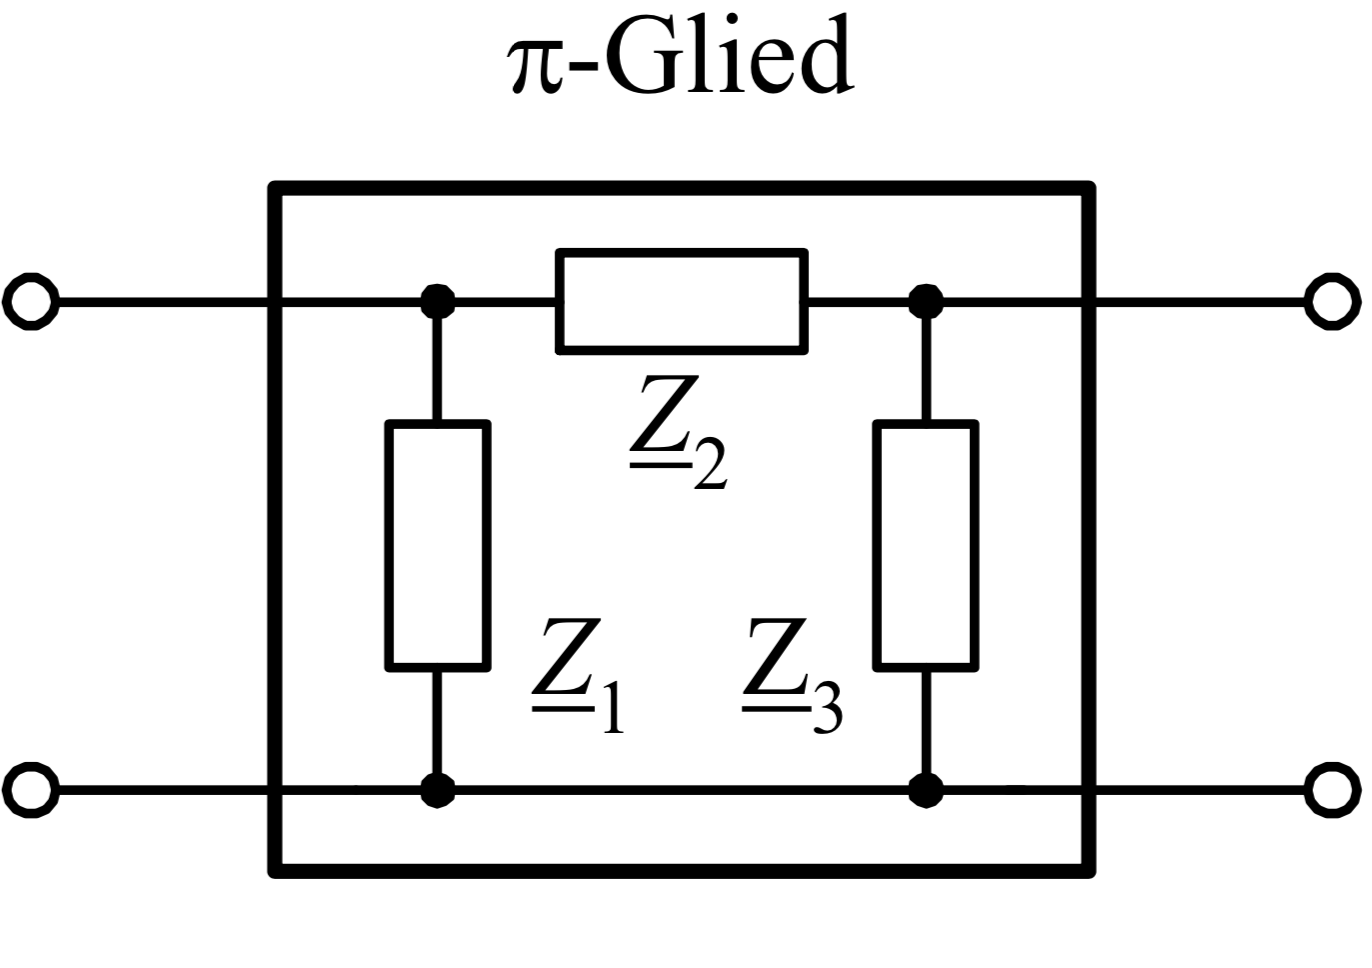
\includegraphics[width = 3cm]{pi_impedance.png}
		\label{fig:piImpedance}
		\caption{Pi-Glied}
	\end{minipage}
	\begin{minipage}[h]{0.45\linewidth}
		\begin{equation}\label{equ:piImpedance}
			A_\pi = \left[\begin{matrix}
			1+\frac{\underline{Z}_2}{\underline{Z}_3}&\underline{Z}_2\\
			\frac{1}{\underline{Z}_1}+\frac{1}{\underline{Z}_3}+\frac{\underline{Z}_2}{\underline{Z}_1\underline{Z}_3}&1+\frac{\underline{Z}_2}				{\underline{Z}_1}
			\end{matrix}\right]
		\end{equation}
	\end{minipage}
\end{figure}

Wenn die ABCD-Matrix einer Schaltung gebildet wurde, kann diese direkt in die Streuparameter umgewandelt werden. Der $s_{21}$ Parameter kann wie in Formel \ref{equ:s21} beschrieben, durch einsetzten der ABCD-Matrix bestimmt werden.
\begin{equation}\label{equ:s21}
s_{21} = \frac{2}{A_{11}+\frac{A{12}}{R_w}+A_{21}*R_w+A_{22}}
\end{equation}
\newpage

\subsection{Berechnungsbeispiel} \label{subsec:beispiel}
Folgender Abschnitt zeigt auf, wie die Einfügungsverluste ermittelt werden. Als Beispielschaltung wird das CM-Schaltungsäquivalent verwendet. Die Schaltung beinhaltet eine Queradmittanz und eine Längsimpedanz, welche in Schritt 1 \ref{subsubsec:schritt1} zusammengefasst werden. Im Schritt 2 werden diese dann in die ABCD-Matrixen(Kettenmatrixen) eingesetzt. Durch kaskadieren der einzelnen Kettenmatrixen wird in Schritt 3 die Kettenmatrix der kompletten Schaltung erstellt. Diese Kettenmatrix kann nun zusammen mit dem Bezugswiderstand in die Definition des Streuparameters $s_{21}$ eingesetzt werden (Schritt 4).

\begin{figure}[H]
	\begin{minipage}[h]{0.45\linewidth}
		\centering
		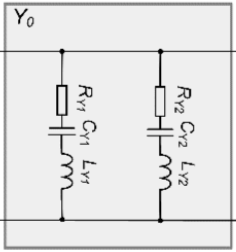
\includegraphics[width=3.5cm]{CM_Admittanz.png}
		\label{fig:CM-Admittanz}
		\caption{CM-Admittanz}
	\end{minipage}
	\hfill
	\begin{minipage}[h]{0.45\linewidth}
	\centering
		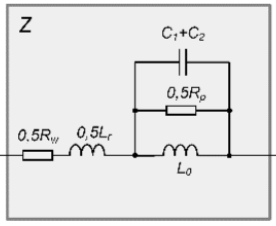
\includegraphics[width=4.5cm]{CM_Impedanz.png}
		\caption{CM-Impedanz}
		\label{fig:CM-Impedanz}
	\end{minipage}
\end{figure}
\subsubsection{Schritt 1: Berechnen der Längsimpedanz Z und der Queradmittanz Y0}\label{subsubsec:schritt1}
Für die Querimpedanz Y0 ergibt sich die Formel
\begin{equation}\label{y_admittance}
Y_0 = \frac{ 1 }{R_{Y1} + \frac{1}{j*\omega*C_{Y1}}+j*\omega*L_{Y1}} +\frac{ 1 }{R_{Y2} + \frac{1}{j*\omega*C_{Y2}}+j*\omega*L_{Y2}}
\end{equation}

Für die Längsimpedanz ergibt sich folgende Formel
\begin{equation}\label{z_impedance}
Z = 0.5*R_w+j*\omega*L_r+\frac{ 1 }{ \frac{1}{0.5*R_p}+j*\omega*L_r*(C_1+C_2)+\frac{1}{j*\omega*L_0} }
\end{equation}

\subsubsection{Schritt 2: Erstellen der ABCD-Matrixen}\label{subsubsec:schritt2}

Somit ergeben sich die ABCD-Matrixen wie folgt
\begin{equation}\label{equ:abcd_a1}
A_1 =
\left[\begin{matrix}
1 & 0\\ Y&1 
\end{matrix}\right]
\end{equation}
\begin{equation}\label{equ:abcd_a2}
A_2 =
\left[\begin{matrix}
1 & Z\\ 0&1 
\end{matrix}\right]
\end{equation}

\subsubsection{Schritt 3: Gesamt-Kettenmatrix bilden}\label{subsubsec:schritt3}
Die ABCD-Matrixen haben den Vorteil, dass man sie sehr unkompliziert kaskadieren kann indem man das Produkt bildet.
\begin{equation}
A = A_1*A_2 = A_2 = \left[\begin{matrix}
1 & 0\\ Y&1 
\end{matrix}\right] * 
\left[\begin{matrix}
1 & Z\\ 0&1 
\end{matrix} \right]
\end{equation}

\subsubsection{Schritt 4: S21 Parameter bilden}\label{subsubsec:schritt4}
Der S21 Parameter ist wie folgt definiert.
\begin{equation}\label{equ:def_s21_aparams}
S_{21} = \frac{2}{A_{11}+\frac{A{12}}{R_w}+A_{21}*R_w+A_{22}}
\end{equation}

Somit sind alle gesuchten Werte gegeben und der S21 Parameter wird durch einsetzen der Werte gebildet.

\subsubsection{Schritt 5: Einfügungsverluste bilden}\label{subsubsec:schritt5}
Durch einsetzen des Streuparameters S21 in die Definition der Einfügunsverluste lassen sich diese Darstellen. Folgende Grafik \ref{fig:Vergleich Berechnung Simulation} zeigt die Berechnungen in MATLAB (Mitte) im Direktvergleich mit der Grafik aus der Aufgabenstellung(Links) sowie die Simulation in MPLAB Mindi (Rechts). Die Differenzen lassen sich dadurch erklären, dass in der Aufgabenstellung die Werte der Bauelemente nicht gegeben sind.
\begin{figure}[H]
	\centering
	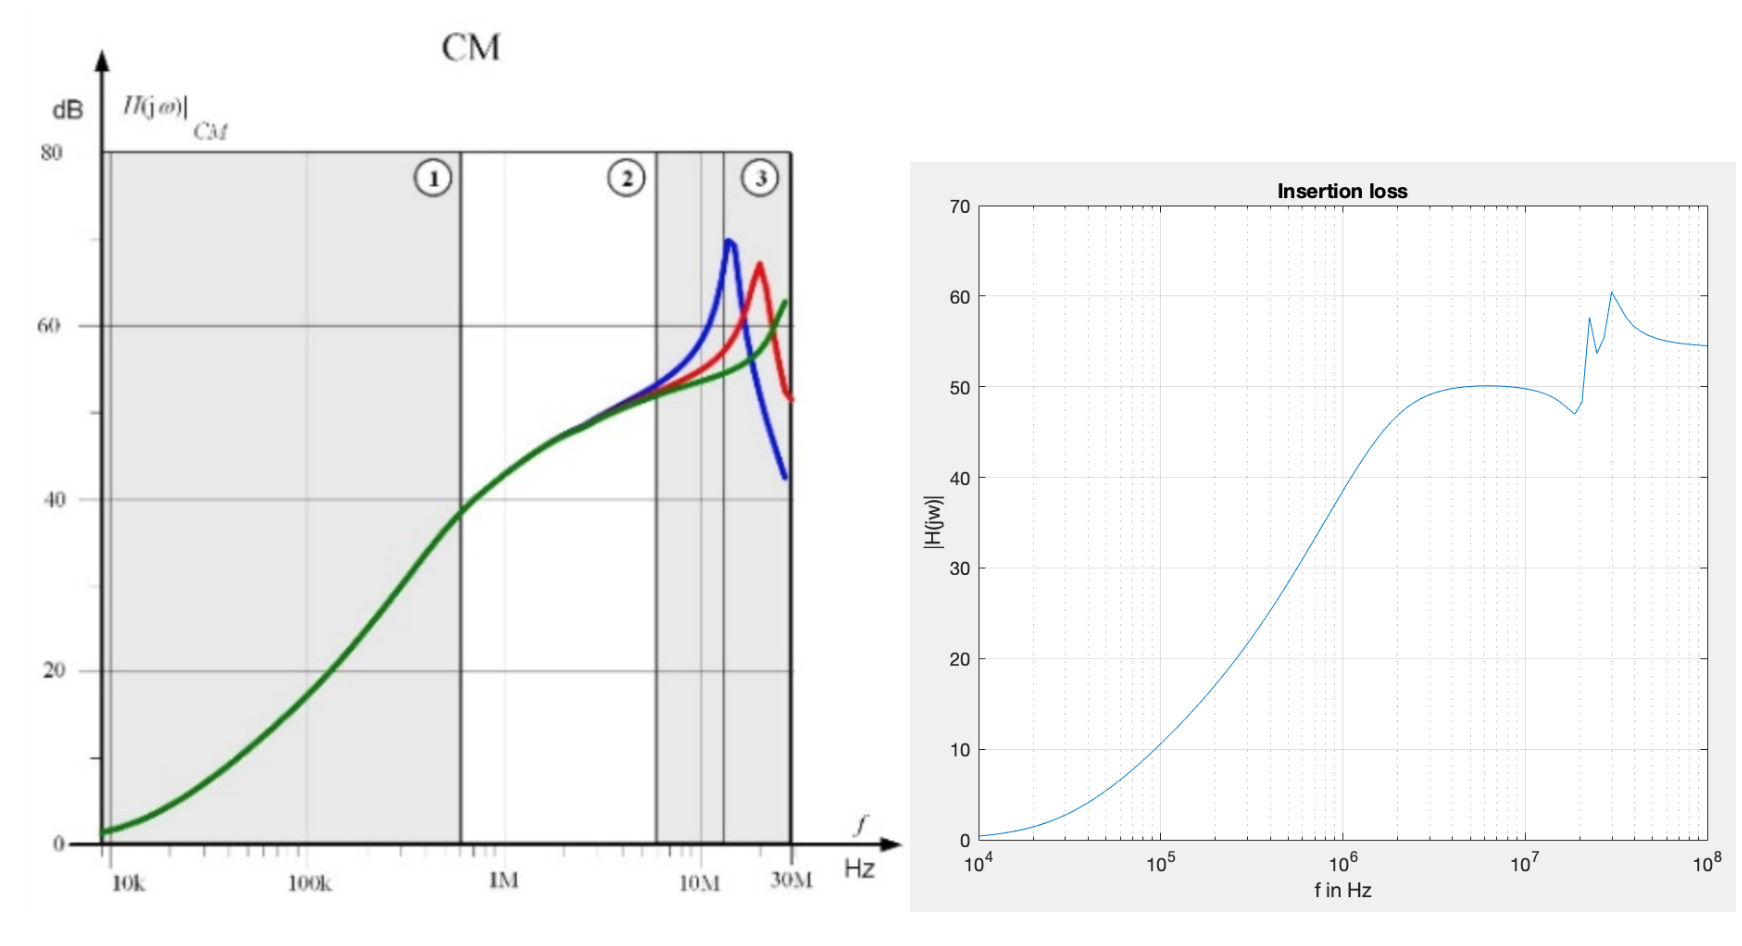
\includegraphics[width=15cm]{CM_vergleich.png}
	\caption{Vergleich Vorgabe/ Berechnung/ Simulation}
	\label{fig:Vergleich Berechnung Simulation}
\end{figure}
